\documentclass[a4paper]{exercisesheet}

%\usepackage{mathpazo}
%\usepackage{mathptmx}
%\usepackage{newtxmath}
\usepackage[T1]{fontenc}
\usepackage[utf8]{luainputenc}
\usepackage[charter]{mathdesign}
\let\sfdefault=\rmdefault
\def\ttdefault{txtt}

\usepackage[dvipsnames]{xcolor}
%\colorlet{maincolor}{blue!50!black}
\colorlet{maincolor}{black}

\usepackage{listings}
%\lstset{
%  frame=lines,
%  backgroundcolor=\color{maincolor!15},
%  rulecolor=\color{maincolor},
%  language=Python
%  keywordstyle=\bfseries\color{maincolor},
%  numbers=left,
%  numberstyle=\scriptsize\color{maincolor!70},
%}

\linespread{1.04}

\usepackage[english]{babel}

\usepackage{blindtext}

\sheetconf{
    lecture   = {Netzwerke und komplexe Systeme},
  lecturer  = {F.~Klimm~und~B.F.~Maier},
  semester  = {Sch\"ulerakademie 5.2 (Ro\ss leben 2016)},
  author    = {},
  % teacher,
  solutions=false,
}

\setsheetfont{lecture on titlepage}{\sffamily\Huge}
\setsheetfont{sheet title}{\sffamily\Large}
\setsheetfont{type on titlepage}{\sffamily\scriptsize\color{maincolor}}
\setsheetfont{sheet topic}{\sffamily\Huge\color{maincolor}}
\setsheetfont{sheet lecture}{\it\sffamily\Large\color{maincolor}}
\setsheetfont{exercise topic}{\sffamily\Large\color{maincolor}}
\setsheetfont{exercise label}{\sffamily\Large\color{maincolor}}
\setsheetfont{subexercise topic}{\sffamily\large\color{maincolor}}
\setsheetfont{subexercise label}{\sffamily\large\color{maincolor}}

\setsheettemplate{sheet title (student)}{Übungsblatt~\thesheet}
\setsheettemplate{exercise name}{Aufgabe}
\setsheettemplate{subexercise name}{Teilaufgabe}

\lstset{%
  %linewidth=\textwidth,
  %linewidth=16cm,
  language=Python,                  % the language of the code
  basicstyle=\ttfamily\small,
  backgroundcolor=\color{maincolor!5},
  %basicstyle=\footnotesize,      % the size of the fonts that are used for the code
  numbers=left,                   % where to put the line-numbers
  stepnumber=1,                   % the step between two line-numbers. If it's 1, each line 
                                  % will be numbered
  numberstyle=\scriptsize\color{maincolor!70},
  numbersep=5pt,                  % how far the line-numbers are from the code
  frame=single,                   % adds a frame around the code
  rulecolor=\color{black},        % if not set, the frame-color may be changed on line-breaks
  tabsize=4,                      % sets default tabsize to 2 spaces
  captionpos=b,                   % sets the caption-position to bottom
  breaklines=true,                % sets automatic line breaking
  breakatwhitespace=false,        % sets if automatic breaks should only happen at whitespace
  %keywordstyle=\color{blue},      % keyword style
  %commentstyle=\color{dkgreen},   % comment style
  %stringstyle=\color{colorNavy},  % string literal style
  morekeywords={*,with, where, from, union, all, as},
  extendedchars=true,
  literate={ä}{{\"{a}}}1 {ö}{{\"o}}1 {ü}{{\"u}}1,
}


\usepackage{pstricks,pst-node,pst-tree}



\begin{document}

  \sheet[%
  number=2,
      topic={F\"arbung von Graphen},
      %deadline=Deadline: \today,
    ]

\vspace{-1cm}
\noindent\rule{12cm}{0.4pt}

  \exercise[%
  topic = Knotenf\"arbung 
    ]

%\lstinputlisting{./code/pfadgraph.py}



 \subexercise[%
  topic=Einen Graphen f\"arben,
    ]

Finde zwei g\"ultige Knotenf\"arbungen f\"ur den abgebildeten Graphen.

\begin{figure}[h]
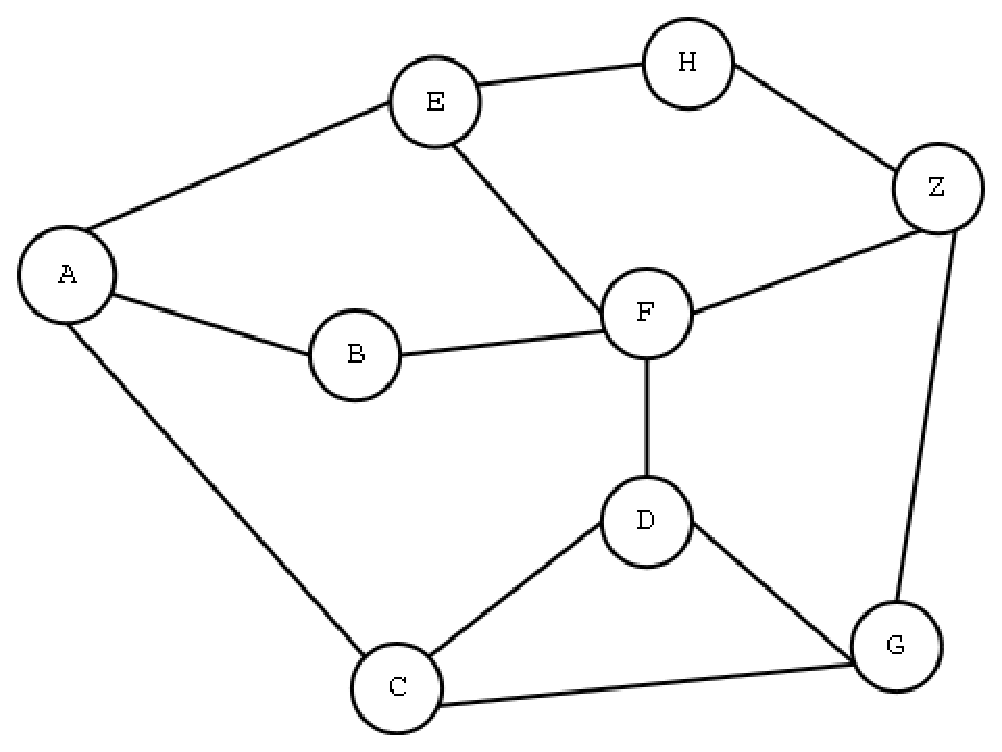
\includegraphics[width=0.4\textwidth]{graph_colouring.eps}
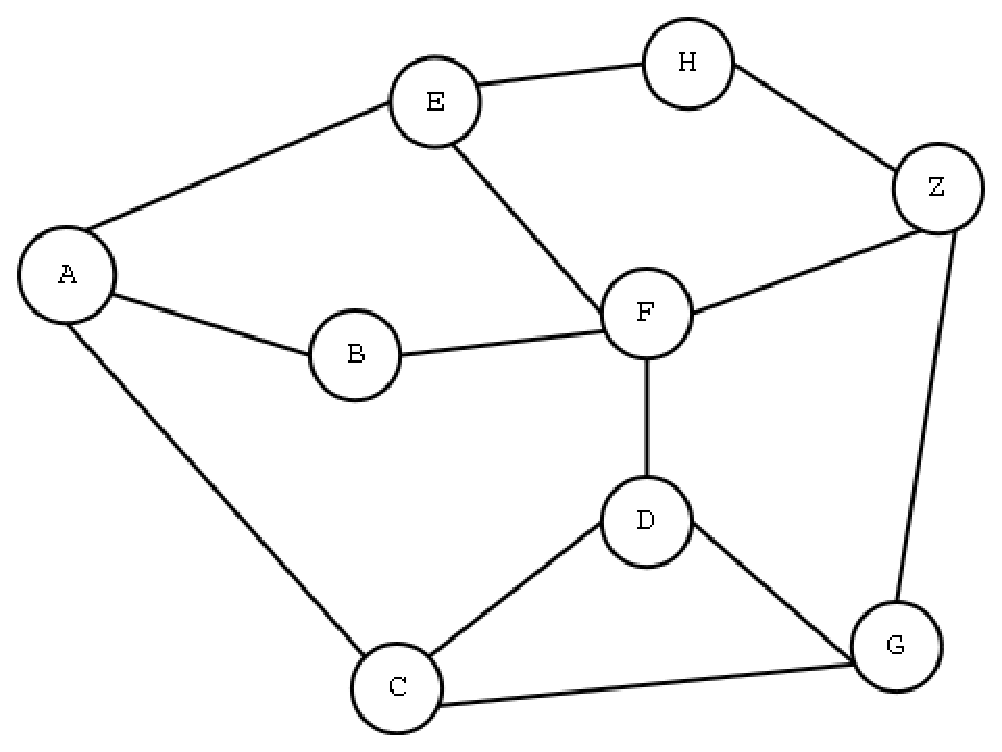
\includegraphics[width=0.4\textwidth]{graph_colouring.eps}
\end{figure}
%\clearpage

Wie viele Farben verwenden diese F\"arbungen?

Finde eine F\"arbung, die eine Farbe mehr verwendet als deine erste F\"arbung.

Was ist die maximal m\"ogliche Anzahl von Farben, die eine F\"arbung verwenden kann?

Finde die minimal m\"ogliche Anzahl von Farben, die eine g\"ultige F\"arbung
ergibt (also die chromatische Zahl $\chi$).

\subexercise[%
  topic=Chromatische Zahl bestimmter Graphen,
    ]
		\label{subseq:graphen}
Finde die chromatische Zahl $\chi$ der folgenden Graphen in Abh\"anigkeit von der Anzahl $n$ der Knoten:
\begin{enumerate}
\item Nullgraph $N_n$
\item Pfadgraph $P_n$
\item Kreisgraph $C_n$
\item Kompletter Graph $K_n$
\item Kompletter bipartiter Graph $K_{n,n}$
\end{enumerate}

\subexercise[%
  topic=Chromatische Zahl,
    ]
Gib zwei nichtisomorphe Beispielgraphen mit 5 Knoten und der chromatischen Zahl 3 an.

\subexercise[%
  topic=Zoodirektor,
    ]
    Ein Zoodirektor m\"ochte die folgenden $5$ Tiere in m\"oglichst wenigen Gehege unterbringen: Adler, Schlange, Maus, L\"owe und Ziege. Finde die minimal n\"otige Anzahl von Gehegen um diese Tiere unterzubringen wenn die folgenden Tiere nicht im selben Gehege sein d\"urfen: Adler \& Schlange, Schlange \& Maus, L\"owe \& Ziege.


\subexercise[%
  topic=Petersen Graph,
    ]
    In Abbildung \ref{petersen} siehst du den sogenannten Petersen Graph. Finde dessen chromatische Zahl $\chi$. Skizziere ihn mit einer $\chi$-F\"arbung.

\begin{figure}[h]
    \centering
    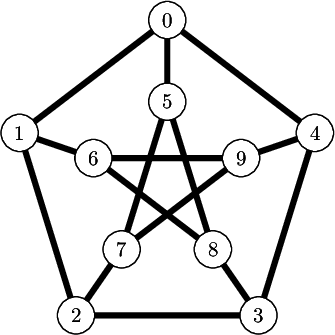
\includegraphics[width=0.4\textwidth]{petersen_graph.eps}
    \caption{\label{petersen} Petersen Graph.}

%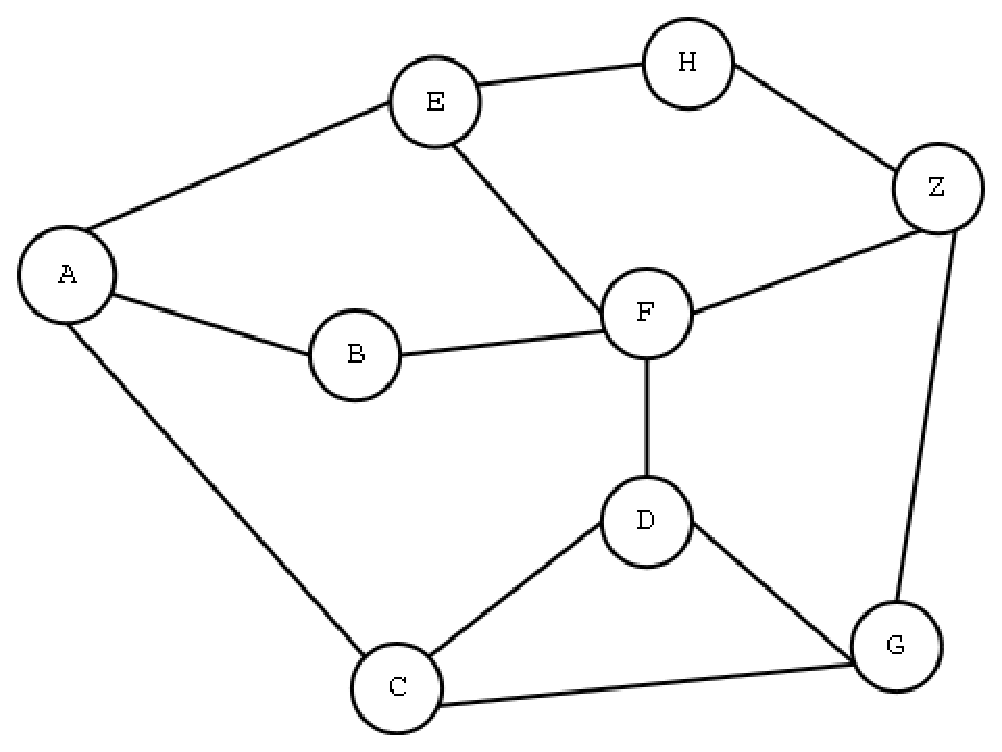
\includegraphics[width=0.4\textwidth]{graph_colouring.eps}
\end{figure}

\subexercise[%
  topic=Eine Obergrenze f\"ur die chromatische Zahl,
    ]
Sei $G$ ein Graph aus $n$ Knoten und {\bf nicht} der komplette Graph $K_n$. Zeige, dass $\chi (G) < n$.
\emph{Hinweis: Es kann n\"utzlich sein zuerst folgendes Lemma zu beweisen: Sei $c(V)$ eine zul\"assige F\"arbung des Graphen $G=(V,E)$. Dann ist $c(V)$ auch eine zul\"assige F\"arbung des Graphen $G'=(V,E')$, wobei $E'\subset E$.}


\subexercise[%
  topic=Graphen gleicher Gr\"o\ss e mit unterschiedlichem Chromatischer Zahl,
    ]
		
		Finde Graphen $G$ und $H$ so dass die Zahl $n$ an Knoten und $m$ der Kanten gleich sind aber $\chi (G)> \chi (H)$.


\exercise[%
  topic = Graphisomorphismus 
    ]
		
		\subexercise[%
  topic=Isomorphie von Graphen untersuchen,
    ]
		
		Welche dieser Graphen sind isomorph? F\"ur jene die isomorph sind konstruiere einen Isomorphismus. F\"ur jene die es nicht sind, finde eine graphentheoretische Gr\"o\ss e die sich bei beiden Graphen unterscheidet.
		\begin{figure}[h]
    \centering
    \includegraphics[width=0.9\textwidth]{isomorphismus.eps}
    \caption{\label{isomorphismus} Welche dieser Graphen sind isomorph?}

%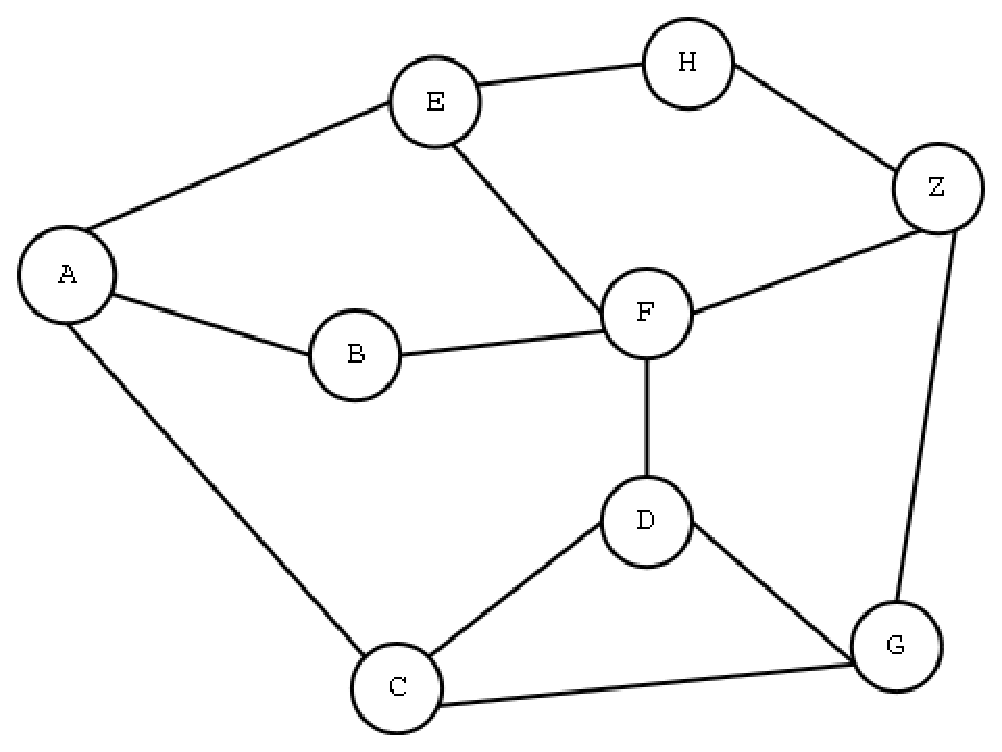
\includegraphics[width=0.4\textwidth]{graph_colouring.eps}
\end{figure}

\subexercise[%
  topic=2-regul\"are Graphen,
    ]
Die Menge aller 2-regul\"aren Graphen kann auch als \emph{Vereinigung von Kreisgraphen} beschrieben werden. Finde verschiedene 2-regul\"are Graphen mit $n=10$. 
Beweise, dass diese Graphen nicht isomorph sind.
\clearpage 
\exercise[%
  topic = Kantenf\"arbung 
    ]

\subexercise[%
  topic=Kantenf\"arbung eines Graphen,
    ]

Finde eine g\"ultige Kantenf\"arbung f\"ur den abgebildeten Graphen welche $\Delta$ Farben verwendet, wobei $\Delta$ sein maximaler Grad ist. Wie ist der chromatische Index dieses Graphen?

\begin{figure}[h]
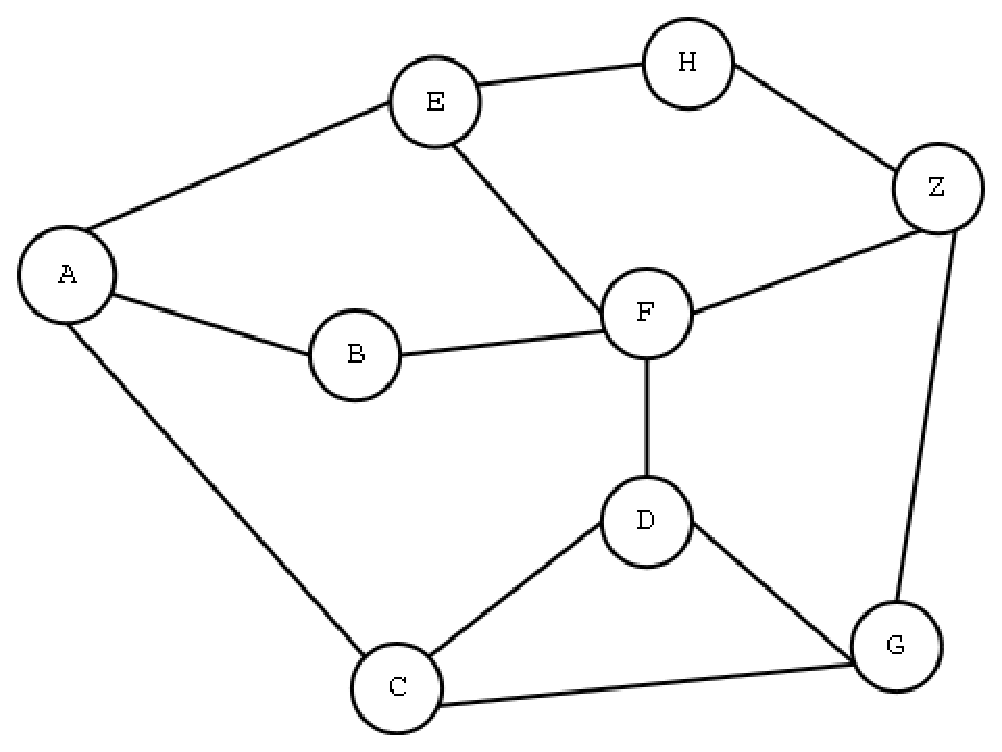
\includegraphics[width=0.4\textwidth]{graph_colouring.eps}
%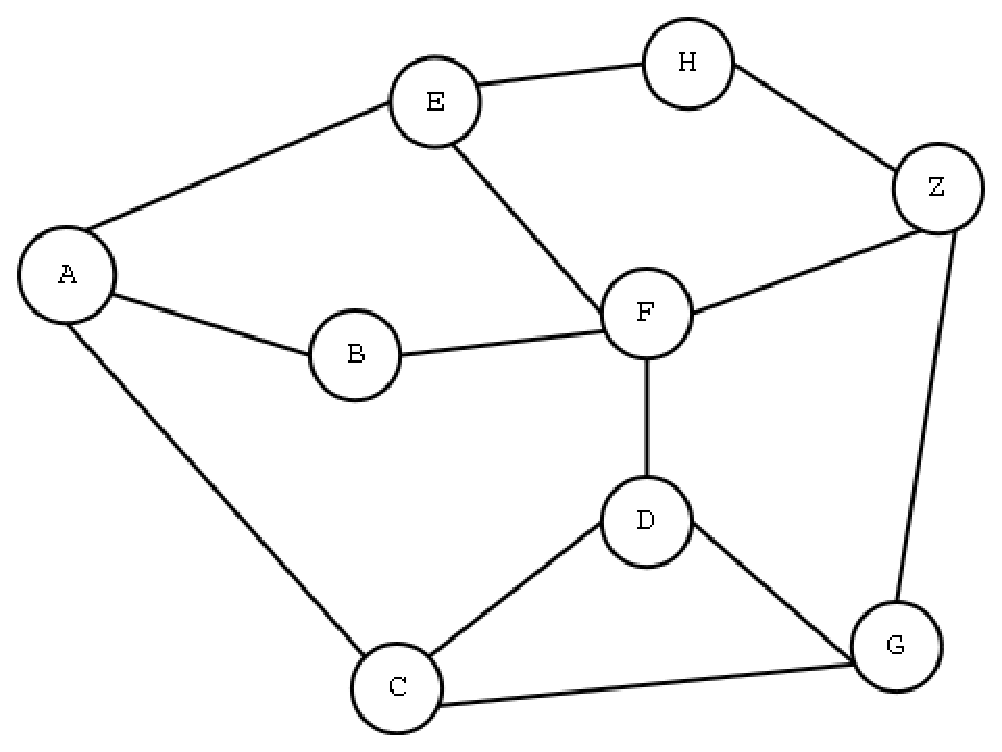
\includegraphics[width=0.4\textwidth]{graph_colouring.eps}
\end{figure}

\subexercise[%
  topic=Kantenf\"arbung bestimmter Graphen,
    ]
Bestimme den chromatischen Index $\chi'$ der folgenden Graphen in Abh\"anigkeit von der Anzahl $n$ der Knoten:

\begin{enumerate}
\item Pfadgraph $P_n$
\item Kreisgraph $C_n$
\item Kompletter Graph $K_n$ (schwierig, eventuell auslassen)
\end{enumerate}

Vergleiche f\"ur diese Graphen den chromatischen Index $\chi$ mit dem maximalen Grad $\Delta$.


\exercise[%
  topic = Gierige F\"arbung Programmieren
    ]

Wir wollen den gierigen F\"arbung-Algorithmus programmieren und auf verschiedene Netzwerke anwenden.
\subexercise[%
  topic=Gierige F\"arbung,
    ]
		Erstelle eine Funktion die als Input eine Adjazenzmatrix und eine Reihenfolge aller Knoten hat und die Knoten des Graphen \emph{gierig} f\"arbt.
\subexercise[%
  topic=Gierige F\"arbung von bestimmten Graphen,
    ]
Wende den gierigen Algorithmus auf die Graphen von Teilaufgabe \ref{subseq:graphen} an wenn $n=10$. Verwende verschiedene zuf\"allige Reihenfolgen der Knoten. Vergleiche deine analytischen Ergebnisse f\"ur die chromatische Zahl mit der Anzahl von verwendeten Farben der gierigen F\"arbung.
		
		
		\subexercise[%
  topic=Zeitkomplexit\"at des gierigen F\"arbe-Algorithmus,
    ]

Wir wollen den gierigen Algorithmus auf zuf\"allige Graphen der Gr\"o\ss e $n$ anwenden. Um sicher die chromatische Zahl eines jeden Graphen zu bestimmen m\"ussen wir alle m\"oglichen Knotenreihenfolgen verwenden.\\
Wieviel Knotenreihenfolgen gibt es in Abh\"anigkeit von $n$? \"uberpr\"ufe die Zeitkomplexit\"at des gierigen Algorithmus numerisch.
		
\exercise[%
  topic=K\"afighaltung von Tieren,
    ]

Lade das Netzwerk mit dem Namen {\tt everglades\textunderscore adjazenz.txt}. Es handelt sich um eine Nahrungskette von Tieren im Everglades Nationalpark in Florida. Die Tiere sind verbunden wenn sie in einer R\"auber-Beute Beziehung stehen. Ein Zoo m\"ochte diese $63$ Tiere halten. Es sollen so wenig wie m\"oglich K\"afige verwendet werden wobei Tiere nicht im selber K\"afig sein d\"urfen wenn eines des andere potentiell isst. In der Datei {\tt everglades\textunderscore namen.txt} sind die Namen der Tiere angegeben.


Formuliere das Problem graphentheoretisch und l\"ose es numerisch. Wende dazu den gierigen F\"arbe-Algorithmus auf zuf\"allige Reihenfolgen der Knoten an. 

\exercise[%
  topic=Chromatisches Polynom,
    ]

Recherchiere das Chromatische Polynom und was ein Baum ist. Beweise, dass das chromatische Polynom des Nullgraphen $\chi_{N_n}(t) =t$, des kompletten Graphen $\chi_{K_n}(t) =t^n$ und eines Baums 

\begin{align}
\chi_{G(t)} = t(t-1)^{n-1}
\end{align}
betr\"agt.

 


	
\end{document}
